\documentclass{beamer}
\usepackage[latin1]{inputenc}
\usetheme{Warsaw}
\title[Dynamically kicking balls]{Dynamically kicking balls with a
Nao}
\author{Inge Becht\\ Maarten de Jonge\\ Richard Pronk}
\institute{University of Amsterdam}
\date{June 24, 2012}
\begin{document}

\begin{frame}
\titlepage
\end{frame}

\begin{frame}{Goal of The Project}
    \begin{itemize}
        \item{Making an omnidirectional, dynamic kick for the Nao}
        \item{Nao plans a kick by making a trade-off between
             accuracy, stability and speed}
        \item{Integrating solution into current Dutch Nao Team code}
    \end{itemize}
\end{frame}

\begin{frame}{What is a Nao?}
    \begin{itemize}
        \item{Humanoid robot}
        \item{Used in the Standard Platform League}
    \end{itemize}
     \begin{figure}[H] 
        \begin{center}
            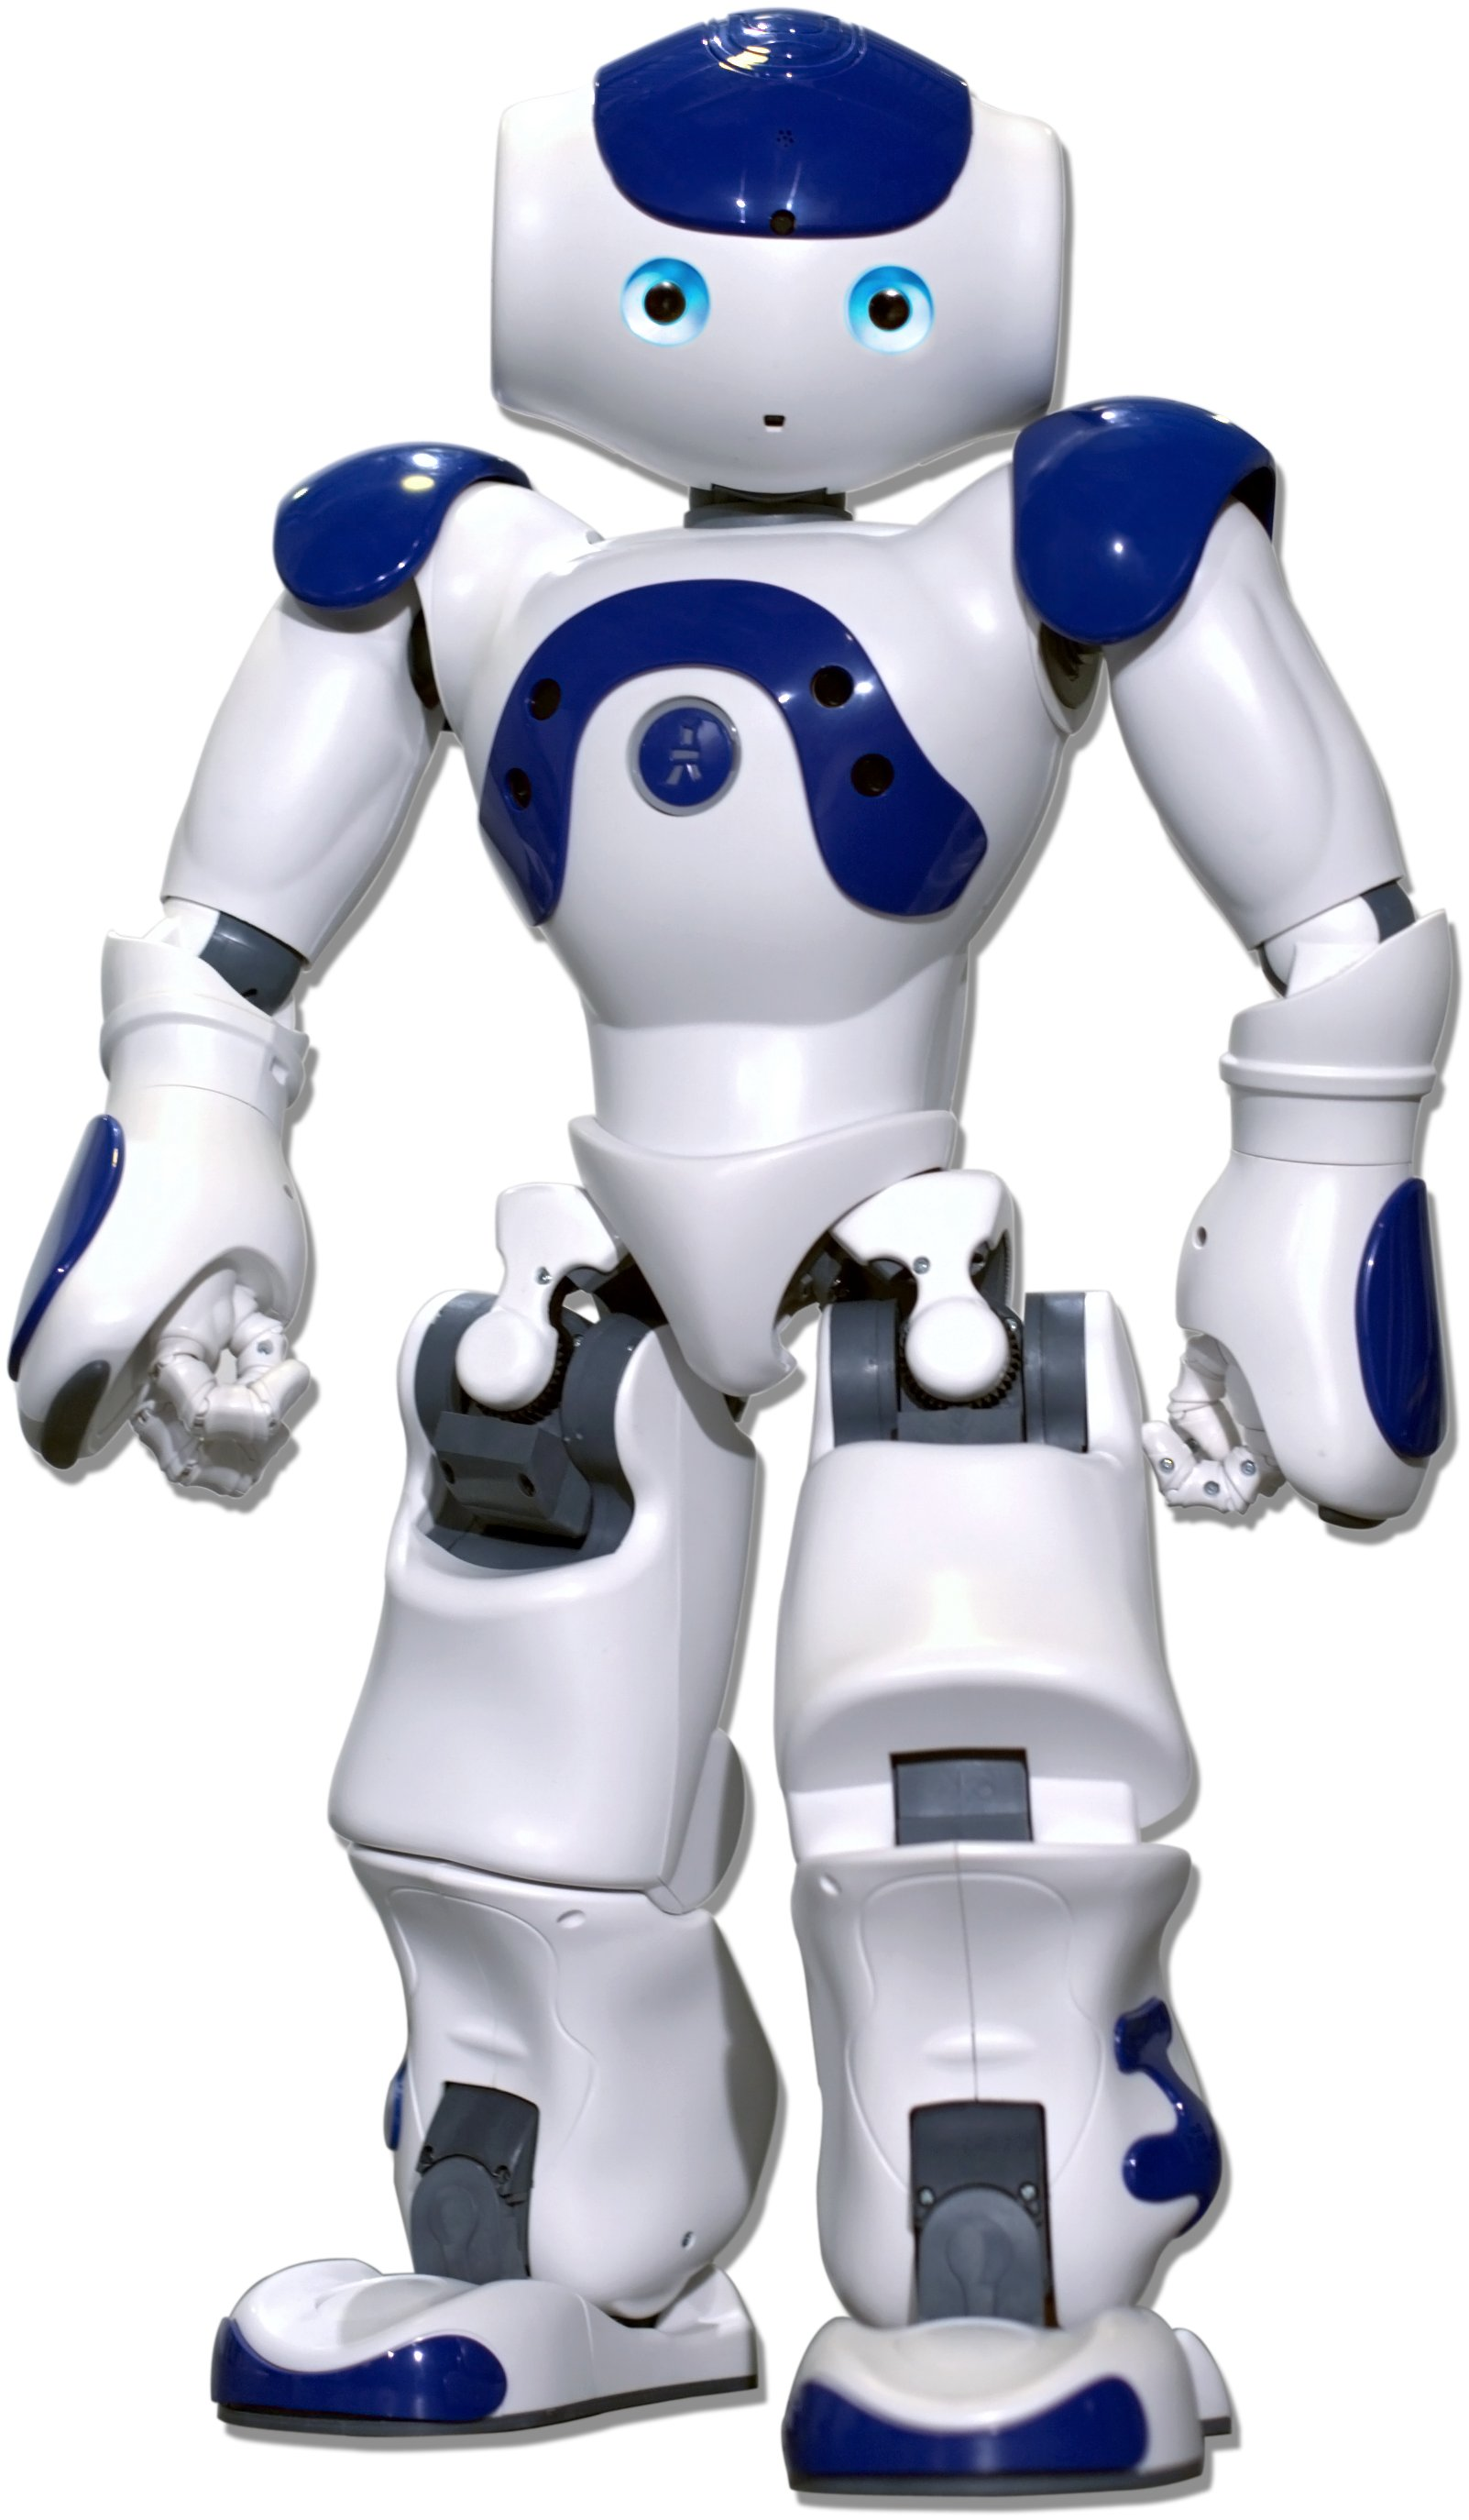
\includegraphics[scale=0.2]{nao.jpg}
            \caption{A Nao robot}
        \end{center}
    \end{figure}  
\end{frame}

\begin{frame}{Why?}
    \begin{itemize}
        \item{Keyframe motions are brittle}
        \item{Able to kick faster and more accurately}
        \item{More robust to environmental factors}
            \begin{itemize}
                \item{Interference by other Naos}
                \item{Compensation for hot joints}
            \end{itemize} 
        \item{Will help the Dutch Nao Team in their next competition}
        \item{Has a large overlap with making a dynamic walk, but is easier}
    \end{itemize}
\end{frame}

\begin{frame}{Possible?}
    \begin{itemize}
        \item{Yes, but quite a lot of work}
        \item{Many topics covered by previous courses}
            \begin{itemize}
                \item{Forward kinematics}
                \item{Inverse kinematics}
            \end{itemize}
        \item{But some further insight is required}
    \end{itemize}
\end{frame}

\begin{frame}{Required Materials and support}
    \begin{itemize}
        \item{Nao available at robolab}
        \item{Team papers about dynamical movement in a Nao} 
        \item{None containing the exact problem we need to tackle}
        \item{We still need to combine the information from the papers and make
            it work for the Nao} 

        \item{Supported by Arnoud Visser}
    \end{itemize}
\end{frame}

\begin{frame}{All tasks}
    \begin{itemize}
        \item{Calculating Center of Mass (Currently working on)}
        \item{Calculating the support polygon}
        \item{Obtaining an inverse kinematics solution}
        \item{Dynamically searching for the optimal kick-trajectory}
    \end{itemize}
\end{frame}

\begin{frame}{Current planning}
    \begin{itemize}
    \item{This week: Calculating Center of Mass on a Nao}
    \item{Two week break: Ola, Mexico!}
    \item{Second week: solving the inverse kinematics chain}
    \item{Third week: Calculating the kick-trajectory}
    \item{Fourth week: wrapping up, integrating with existing code} 
    \end{itemize}
\end{frame}

\end{document}
